\begingroup
\slidenumberfreeheader

\begin{frame}[noframenumbering]{The German Aerospace Center (DLR)}%{Quick facts}

\begin{columns}
\begin{column}{0.4\textwidth}


\tikzstyle{mylocationnodestyle}=[rectangle,draw=none,fill=cyan,inner sep=0.0,minimum size=4pt]
\tikzstyle{mynewlocationnodestyle}=[rectangle,draw=none,preaction={fill=cyan}, pattern=north east lines, pattern color=gray,inner sep=0.0,minimum size=4pt]
\tikzstyle{mylocationlabelstyle}=[inner sep=0.0,font=\tiny]
  
\only<1|handout:1>{
  \begin{tikzpicture}
    \node[anchor=south west,inner sep=0.0] (image) at (0,0) {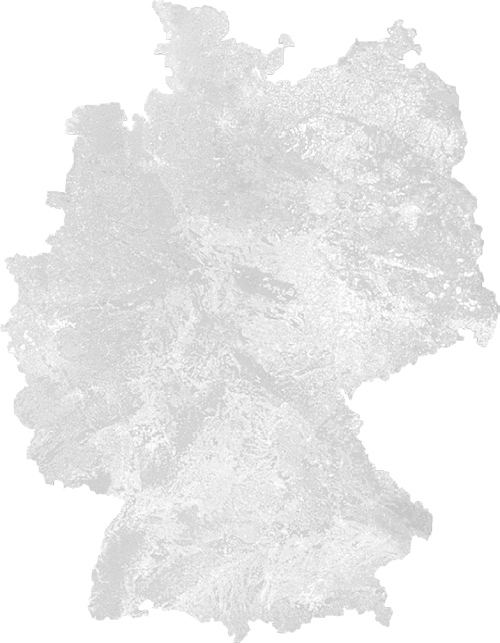
\includegraphics[height=0.85\textheight,width=\linewidth,keepaspectratio]{Germany_bw-ct.png}};
  %   \node[anchor=south west,inner sep=0.0] (image) at (0,0) {\includegraphics[height=0.85\textheight,width=0.5\textwidth,keepaspectratio]{test.png}};
    % Scope
    \begin{scope}[
      x={(image.south east)},
      y={(image.north west)},
    ]
      % Location
      \node[mylocationnodestyle]    (weilheimlocation)         at (0.580,0.085) {};
      \node[mylocationnodestyle]    (oberpfaffenhofenlocation) at (0.592,0.120) {};
      \node[mylocationnodestyle]    (augsburglocation)         at (0.535,0.145) {};
      \node[mylocationnodestyle]    (stuttgartlocation)        at (0.370,0.190) {};
      \node[mylocationnodestyle]    (lampoldshausenlocation)   at (0.397,0.252) {};
      \node[mylocationnodestyle]    (bonnlocation)             at (0.161,0.443) {};
      \node[mylocationnodestyle]    (juelichlocation)          at (0.090,0.471) {};
      \node[mylocationnodestyle]    (koelnlocation)            at (0.144,0.479) {};
      \node[mynewlocationnodestyle] (jenalocation)             at (0.640,0.480) {};
      \node[mynewlocationnodestyle] (dresdenlocation)          at (0.870,0.490) {};
      \node[mylocationnodestyle]    (goettingenlocation)       at (0.459,0.549) {};
      \node[mylocationnodestyle]    (braunschweiglocation)     at (0.514,0.643) {};
      \node[mylocationnodestyle]    (berlinlocation)           at (0.821,0.680) {};
      \node[mylocationnodestyle]    (trauenlocation)           at (0.470,0.726) {};
      \node[mylocationnodestyle]    (bremenlocation)           at (0.325,0.754) {};
      \node[mynewlocationnodestyle] (oldenburglocation)        at (0.260,0.766) {};
      \node[mylocationnodestyle]    (neustrelitzlocation)      at (0.782,0.787) {};
      \node[mynewlocationnodestyle] (bremerhavenlocation)      at (0.300,0.815) {};
      \node[mylocationnodestyle]    (hamburglocation)          at (0.463,0.820) {};
      \node[mylocationnodestyle]    (stadelocation)            at (0.411,0.831) {};
      
      % Location labels
      %\begingroup
      %\fontfamily{lmss}\selectfont
      \node[mylocationlabelstyle, left=0.0em of weilheimlocation] (weilheimlabel) {Weilheim};
      \node[mylocationlabelstyle,right=0.0em of oberpfaffenhofenlocation] (oberpfaffenhofenlabel) {Oberpfaffenhofen};
      \node[mylocationlabelstyle, left=0.0em of augsburglocation] (augsburglabel) {Augsburg};
      \node[mylocationlabelstyle, left=0.0em of stuttgartlocation] (stuttgartlabel) {Stuttgart};
      \node[mylocationlabelstyle,right=0.0em of lampoldshausenlocation] (lampoldshausenlabel) {Lampoldshausen};
      \node[mylocationlabelstyle,right=0.0em of bonnlocation] (bonnlabel) {Bonn};
      \node[mylocationlabelstyle,below left=0.0ex and 0.0em of juelichlocation.south east] (juelichlabel) {J\"ulich};
      \node[mylocationlabelstyle,right=0.0em of koelnlocation] (koelnlabel) {Cologne};%{K\"oln};
      \node[mylocationlabelstyle, left=0.0em of jenalocation] (jenalabel) {Jena};
      \node[mylocationlabelstyle, left=0.0em of dresdenlocation] (dresdenlabel) {Dresden};
      \node[mylocationlabelstyle,right=0.0em of goettingenlocation] (goettingenlabel) {G\"ottingen};
      \node[mylocationlabelstyle, left=0.0em of braunschweiglocation] (braunschweiglabel) {Brunswick};%{Braunschweig};
      \node[mylocationlabelstyle, left=0.0em of berlinlocation] (berlinlabel) {Berlin};
      \node[mylocationlabelstyle,right=0.0em of trauenlocation] (trauenlabel) {Trauen};
      \node[mylocationlabelstyle,below=0.0em of bremenlocation] (bremenlabel) {Bremen};
      \node[mylocationlabelstyle, left=0.0em of oldenburglocation] (oldenburglabel) {Oldenburg};
      \node[mylocationlabelstyle, left=0.0em of neustrelitzlocation] (neustrelitzlabel) {Neustrelitz};
      \node[mylocationlabelstyle, left=0.0em of bremerhavenlocation] (bremerhavenlabel) {Bremerhaven};
      \node[mylocationlabelstyle,right=0.0em of hamburglocation] (hamburglabel) {Hamburg};
      \node[mylocationlabelstyle,above=0.0em of stadelocation] (stadelabel) {Stade};
      %\endgroup
      % Help grid and labels
  %     \draw[help lines,xstep=.1,ystep=.1] (0,0) grid (1,1);
  %     \foreach \x in {0,1,...,9} {\node [anchor=north] at (\x/10,0) {0.\x};}
  %     \foreach \y in {0,1,...,9} {\node [anchor=east]  at (0,\y/10) {0.\y};}
    \end{scope}
  \end{tikzpicture}
}
  
\only<2|handout:0>{
  \begin{tikzpicture}
    \node[anchor=south west,inner sep=0.0] (image) at (0,0) {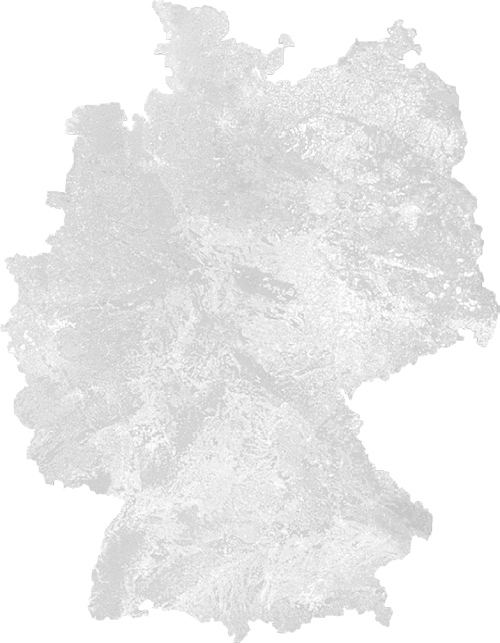
\includegraphics[height=0.85\textheight,width=\linewidth,keepaspectratio]{Germany_bw-ct.png}};
    % Scope
    \begin{scope}[
      x={(image.south east)},
      y={(image.north west)},
    ]
      % Location
      \node[mylocationnodestyle]    (braunschweiglocation)     at (0.514,0.643) {};
      
      % Location labels
      \node[mylocationlabelstyle,font=\footnotesize, left=0.0em of braunschweiglocation] (braunschweiglabel) {Brunswick};%{Braunschweig};
      
      % Subimage
      \node[inner sep=0.0,anchor=north] (bsimage) at (0.5,0.55) {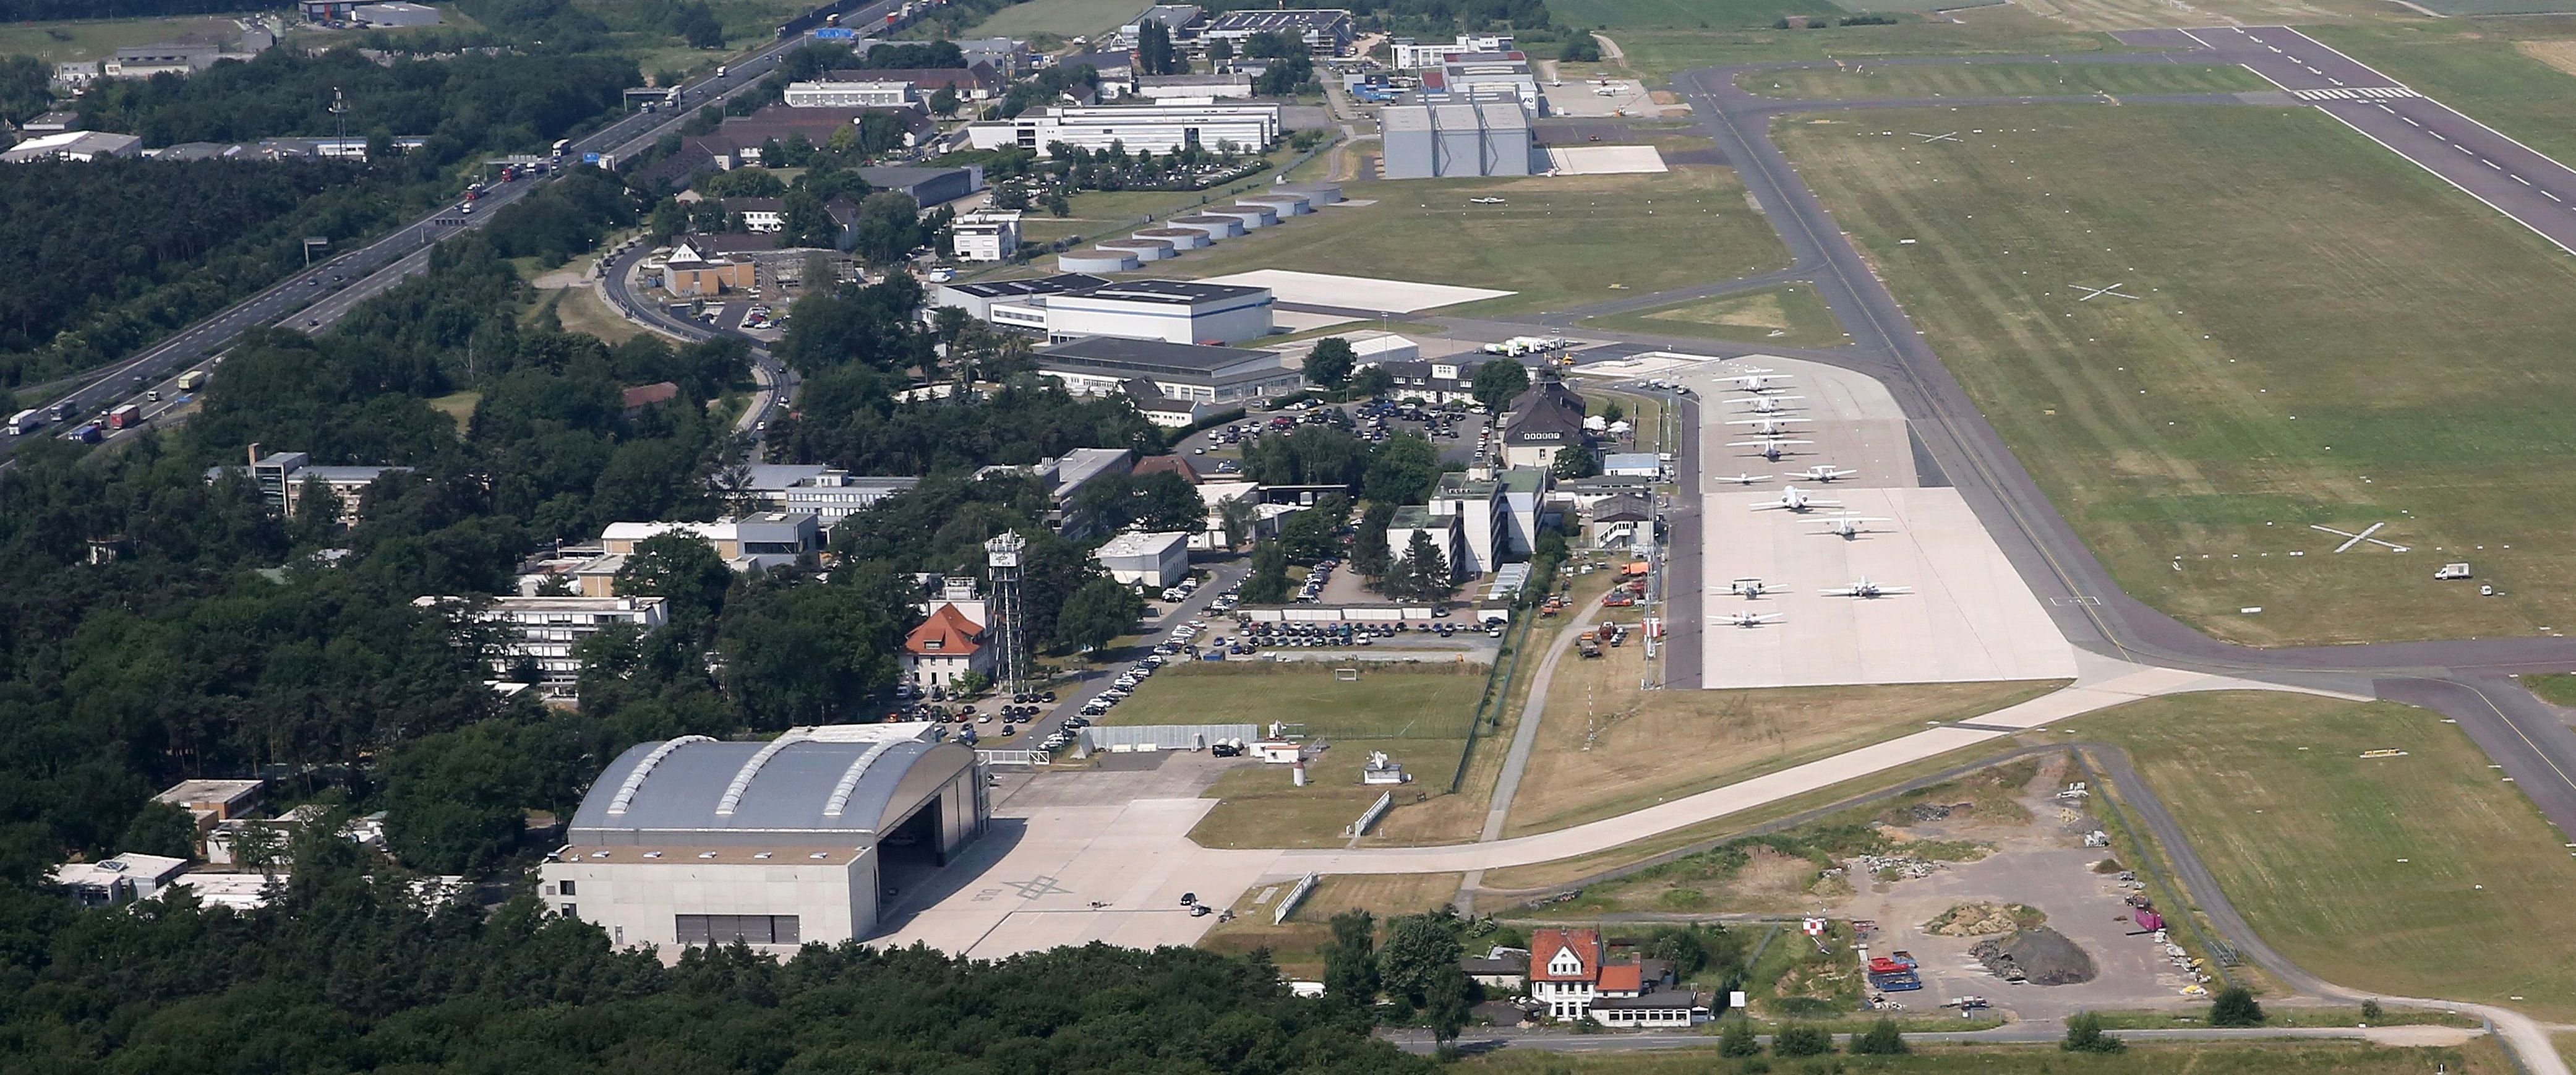
\includegraphics[height=0.4\textheight,width=0.9\linewidth,keepaspectratio]{DLR_BS_c.jpg}};
    \end{scope}
  \end{tikzpicture}
}

% \only<3|handout:0>{
%   \begin{tabularx}{\linewidth}{X}
%     \includegraphics[width=\linewidth, height=0.275\textheight]{example-image-a}\\
%     \includegraphics[width=\linewidth, height=0.275\textheight]{example-image-a}\\
%     \includegraphics[width=\linewidth, height=0.275\textheight]{example-image-a}
%   \end{tabularx}
% }
  
\end{column}
\begin{column}{0.59\textwidth}
  \only<1|handout:1>{
    \begin{block}{Quick facts}
      \begin{itemize}[noitemsep]
        %\item National center for aerospace, energy, security \& transportation research and space agency
        \item National aeronautics and space research centre \& space agency
        \item Research focus: aeronautics, space, energy, transport \& security
        \item 16 locations + 4 new in 2017
        \item 33 institutes
        \item 8000 employees
        \item International offices: Brussels, Paris, Tokyo \& Washington D.C.
      \end{itemize}
    \end{block}
  }
  \only<2|handout:0>{
    \begin{block}{Site Brunswick}
      \begin{itemize}[noitemsep]
        \item 6 institutes
        \item 1100 employees
        \item Wind tunnels, HPC-cluster, flight operations
      \end{itemize}
    \end{block}
    \begin{block}{Institute for Composite Structures \& Adaptive Systems}
      \begin{itemize}[noitemsep]
        \item Focus: adaptable, efficient, robust high-performance composite structures along the entire value chain
        \item Department Structural Mechanics
      \end{itemize}
    \end{block}
  }
%   \only<3|handout:0>{
%     \begin{block}{Department Structural Mechanics}
%       \begin{itemize}[noitemsep]
%         \item Test
%       \end{itemize}
%     \end{block}
%   }

\end{column}
\end{columns}

\end{frame}
\endgroup